\begin{figure}[htb!]
\centering
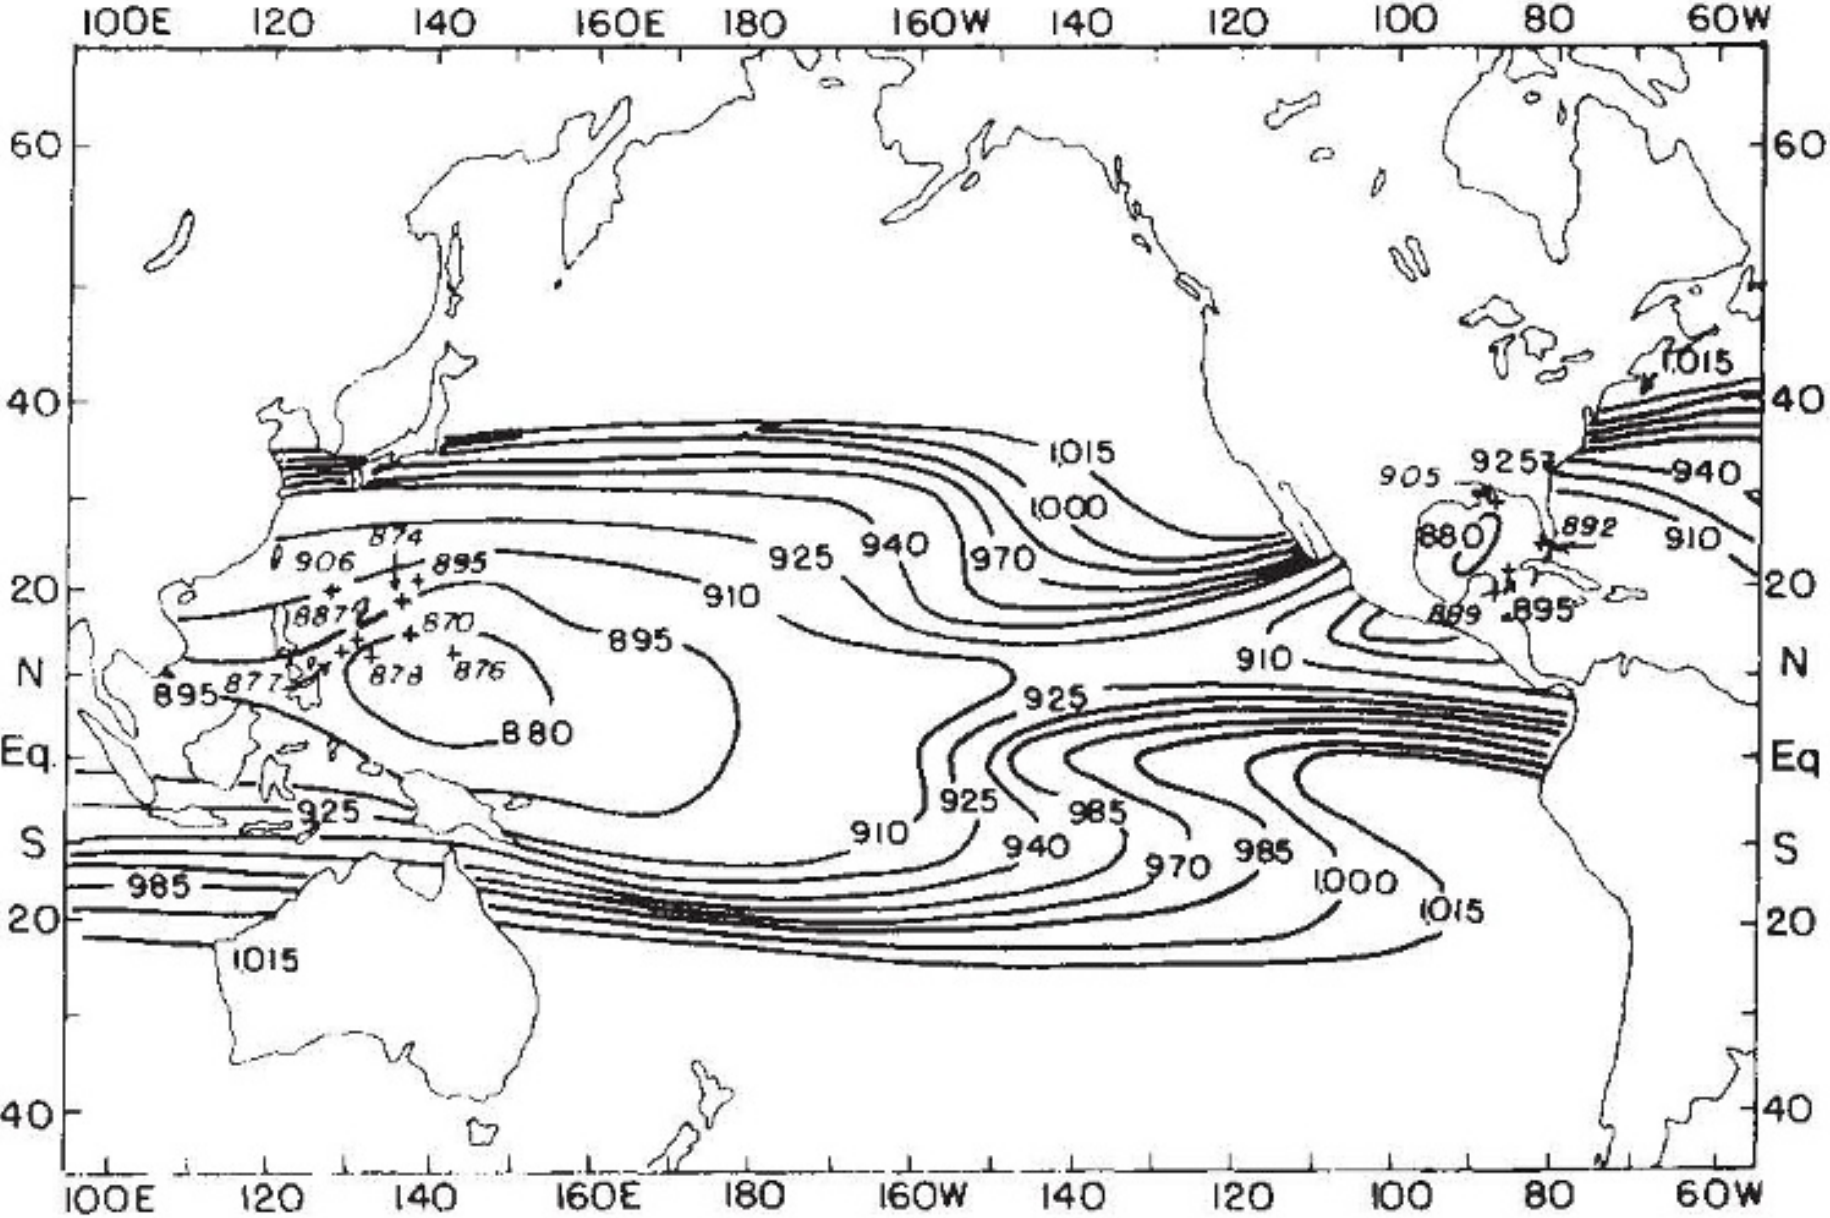
\includegraphics[width=1\linewidth]{images/e87-slimmed-verif.png}\\
\textit{Figure 2 from Emanuel, Nature, 1987~\cite{emanuel1987dependence}}
\caption{minimum sustainable central pressures (mb) under September mean
climatological conditions, assuming an ambient pressure of 1,015 mb~\cite{emanuel1986air}.
Crosses mark the positions and central pressures of some of the most intense
tropical cyclones on record~\cite{anthes2016tropical}.
The data shows that at the time the minimum central pressure
closely matches the limits predicted~\cite{emanuel1986air}. }
\label{fig:emanuel87}
\end{figure}
